% PatoSim: novidades e guia de uso. Fonte editável de docs/PatoSim_novidades.pdf.
% Para gerar o PDF de novo:  ./docs/manual/compilar_pdf.sh   (latexmk + pdflatex)
% Figuras em docs/manual/figuras/ (feitas com gravações e testes reais).
\documentclass[10pt,a4paper]{article}
\usepackage[utf8]{inputenc}
\usepackage[T1]{fontenc}
\usepackage[brazil]{babel}
\usepackage{lmodern}
\usepackage[a4paper,margin=1.9cm]{geometry}
\usepackage{graphicx}
\usepackage{booktabs}
\usepackage{tabularx}
\usepackage{float}
\usepackage[font=small,labelfont=bf]{caption}
\usepackage{xcolor}
\usepackage[hidelinks]{hyperref}
\usepackage{xurl}
\usepackage{enumitem}
\usepackage{listings}
\usepackage{makecell}
\usepackage{tikz}
\usetikzlibrary{arrows.meta,positioning}
\setlist{nosep,leftmargin=1.2em}
\graphicspath{{figuras/}}
\definecolor{cinza}{HTML}{52514e}
\definecolor{fundo}{HTML}{f4f4f2}
\definecolor{azul}{HTML}{2a6f97}
\definecolor{novo}{HTML}{1b7f5b}
\lstset{basicstyle=\ttfamily\small,backgroundcolor=\color{fundo},frame=none,columns=fullflexible,
        keepspaces=true,breaklines=true,showstringspaces=false,xleftmargin=4pt,aboveskip=4pt,belowskip=4pt,
        literate={á}{{\'a}}1 {é}{{\'e}}1 {í}{{\'i}}1 {ó}{{\'o}}1 {ú}{{\'u}}1 {ã}{{\~a}}1 {õ}{{\~o}}1
                 {ç}{{\c{c}}}1 {â}{{\^a}}1 {ê}{{\^e}}1 {ô}{{\^o}}1 {à}{{\`a}}1}
\setlength{\parskip}{4pt}
\setlength{\parindent}{0pt}
\newcommand{\arq}[1]{\texttt{#1}}
% nome longo que pode quebrar em qualquer ponto (xurl)
\newcommand{\nome}[1]{\nolinkurl{#1}}
\newcommand{\botao}[1]{\textbf{#1}}
\newcommand{\novo}{\textcolor{novo}{\textbf{novo}}}
\newcolumntype{Y}{>{\raggedright\arraybackslash}X}

\title{\textbf{PatoSim}\\[2pt]
\large Novidades de outubro e novembro de 2026 e guia de uso\\
\normalsize navegação leve, World Builder, sensores subaquáticos e instalação em outras máquinas}
\author{PDI-DL \textendash{} \url{https://github.com/PDI-DL/PatoSIM} (branch \texttt{main})}
\date{9 de novembro de 2026}

\begin{document}
\maketitle
\vspace{-1.2em}

\section*{Resumo}
O PatoSim é uma extensão do Isaac Sim 5.1 para simular um ROV (BlueROV) e gravar dados de câmera, sonar,
LiDAR, DVL e barômetro. Ele junta a estrutura de gravação do MobilityGen (registro de robôs e cenários,
gravação em duas fases, \arq{Reader}/\arq{Writer}) aos sensores subaquáticos do OceanSim.
O que mudou:
\begin{itemize}
  \item \textbf{Navegação leve} (\novo): todos os sensores começam desligados. Pilotar o ROV pelo mundo fica
        fluido, e cada gravação liga só os sensores de que precisa (seção~\ref{sec:sensores}).
  \item \textbf{World Builder} (\novo): um segundo launcher, sem robô, que carrega o mundo, insere objetos do
        dataset e confere/aplica as classes semânticas, a refletividade do sonar e as colisões antes da
        gravação (seção~\ref{sec:wb}).
  \item \textbf{Sensores}: sonar no modo \texttt{raw} (mantém a queda real de intensidade com a distância) e
        salvo durante a gravação; LiDAR com alcance e atenuação de scanners subaquáticos; teleoperação por
        gamepad em 6 graus de liberdade; extrínsecos dos sensores gravados; mapa de ocupação em camadas de
        profundidade (seção~\ref{sec:detalhes}).
  \item \textbf{Funciona em outras máquinas} (\novo): o código do OceanSim agora vem sempre do próprio repositório
        (\arq{omni.ext.patosim.oceansim}). Antes ele podia vir de uma cópia antiga em \arq{app/extsUser}. Foram
        removidos os caminhos fixos de uma máquina (assets, mundo de exemplo, link \arq{isaacsim/oceansim}, testes).
  \item \textbf{Instalado e testado na pdi\_mini\_3} (RTX 5060 Ti) com o mesmo procedimento do README. Nela e nesta
        máquina (RTX 4070) passam os 32 testes unitários e os testes de integração com o Isaac, exceto o do sinal
        do sonar (seção~\ref{sec:testes}).
\end{itemize}

\begin{figure}[H]
\centering
\begin{tikzpicture}[
  caixa/.style={draw=azul,line width=0.7pt,rounded corners=3pt,fill=azul!6,align=left,
                text width=3.65cm,inner sep=5pt,font=\small},
  seta/.style={-{Stealth[length=2.6mm]},line width=0.8pt,draw=cinza}]
\node[caixa] (wb) {\textbf{1. World Builder}\\\texttt{launch\_world\_builder.sh}\\carregar o mundo sem robô;
  inserir objetos; checar/aplicar classes, refletividade e colisão};
\node[caixa,right=0.55cm of wb] (ps) {\textbf{2. PatoSim}\\\texttt{launch\_patosim.sh}\\\botao{Build}; pilotar
  (sensores desligados); ligar os sensores; \botao{Start/Stop Recording}};
\node[caixa,right=0.55cm of ps] (rp) {\textbf{3. Replay offline}\\\texttt{replay\_directory.py}\\renderiza
  câmera, profundidade, segmentação, sonar e nuvem de pontos};
\node[caixa,right=0.55cm of rp] (dd) {\textbf{4. Dados}\\\texttt{\textasciitilde/PatoSimData}\\\arq{Reader},
  Gradio, \texttt{sonar\_viz.py}, LeRobot};
\draw[seta] (wb) -- (ps); \draw[seta] (ps) -- (rp); \draw[seta] (rp) -- (dd);
\end{tikzpicture}
\caption{Fluxo de trabalho. O passo 1 é opcional para mundos já preparados; o Build do passo 2 também aplica
colisão e refletividade padrão.}
\end{figure}

%-------------------------------------------------------------------------------------------------------------
\section{Instalação}\label{sec:instalacao}

\subsection{Máquina nova}
Pré-requisitos: Ubuntu com GPU NVIDIA RTX e o \textbf{Isaac Sim 5.1.0} (pacote standalone extraído, por exemplo em
\arq{\textasciitilde/isaacsim}). Os comandos rodam na raiz do repositório.
\begin{lstlisting}[language=bash]
git clone https://github.com/PDI-DL/PatoSIM.git PatoSim && cd PatoSim
./link_app.sh --path ~/isaacsim                 # cria app/ -> Isaac Sim
./app/python.sh -m pip install tqdm wheel        # dependências no Python do Isaac
cd path_planner
../app/python.sh -m pip install pybind11
../app/python.sh -m pip install --no-build-isolation -e .   # planejador em C++
cd ..
python3 -m pip install huggingface_hub hf_transfer        # qualquer Python 3
python3 scripts/assets/downloadAll.py                    # assets -> assets/models
\end{lstlisting}
Os assets (mundos, modelo do BlueROV e objetos do dataset) estão no dataset público \arq{PDI-DL/PatoSimAssets} do
Hugging Face. O \arq{downloadAll.py} os coloca em \arq{assets/models/}. O \arq{scripts/assets/assets.sh} trabalha com
um clone git do dataset privado \arq{PDI-DL/PDI\_3DUW} e precisa de login com acesso a ele. O PatoSim também os encontra direto em \arq{assets/}
(\arq{worlds/}, \arq{bluerov/}, \arq{plataforms/}, \arq{statues\_temples/}, \arq{scenario/}), que é o layout da pdi\_mini\_3.

\subsection{Atualizar uma máquina que já tem o PatoSim}
Foi o que se fez na pdi\_mini\_3 em 09/11/2026. A cópia dela estava na branch \arq{update\_imports}, que agora faz
parte do \arq{main}. Os assets em \arq{assets/}, fora do git, não são tocados.
\begin{lstlisting}[language=bash]
cd ~/Documents/PatoSIM
git fetch origin && git switch main && git pull --ff-only
./app/python.sh -m pip install tqdm wheel
cd path_planner && ../app/python.sh -m pip install pybind11 \
  && ../app/python.sh -m pip install --no-build-isolation -e . && cd ..
\end{lstlisting}
O \arq{path\_planner} é recompilado no último comando. Confira com os testes da seção~\ref{sec:testes} ou com
\begin{lstlisting}[language=bash]
./app/python.sh -c "import tqdm, mobility_gen_path_planner; print('ok')"
\end{lstlisting}

\subsection{Abrir}
\begin{lstlisting}[language=bash]
./scripts/launch_patosim.sh         # simulador: robô, sensores, gravação
./scripts/launch_world_builder.sh   # World Builder: só o mundo, sem robô
\end{lstlisting}
Variáveis opcionais: \arq{PATOSIM\_DATA} (pasta dos dados, padrão \arq{\textasciitilde/PatoSimData}),
\arq{PATOSIM\_DEV\_SCENE} (mundo do botão \botao{Use MHL Scene}, padrão \arq{worlds/Prototipo1/world.usd} dos assets) e
\arq{PATOSIM\_ROV\_WAYPOINTS} (arquivo de waypoints do cenário de waypoints).

%-------------------------------------------------------------------------------------------------------------
\section{Usar o simulador}\label{sec:uso}

\subsection{Montar o cenário}
Na janela \textbf{PatoSim}:
\begin{enumerate}[leftmargin=1.6em]
  \item \botao{Use MHL Scene} preenche \textbf{USD Path / URL} com o mundo de exemplo. Para outro mundo, cole o
        caminho do \arq{.usd}.
  \item \textbf{Scenario Type}: \nome{OceanSimROVTeleoperationScenario} (teclado),
        \nome{OceanSimROVGamepadTeleoperationScenario}, \nome{OceanSimROVWaypointScenario} ou
        \nome{OceanSimROVPathFollowingScenario}. \textbf{Robot Type}: \arq{OceanSimROVRobot}.
  \item Em \botao{Robot Setup}, marque os sensores (se for gravar) e ajuste velocidades e profundidade.
  \item \botao{Build}. Em alguns segundos aparecem o mundo, o ROV e o mapa de ocupação. \botao{Reset} reposiciona o robô.
\end{enumerate}

\begin{table}[H]
\centering\small
\begin{tabularx}{\textwidth}{@{}lY@{}}
\toprule
Botão / campo & O que faz \\
\midrule
\botao{Build}, \botao{Reset} & monta o cenário com o mundo, o robô e os sensores marcados; reposiciona o robô \\
\botao{Start Recording} / \botao{Stop Recording} & grava em \arq{\textasciitilde/PatoSimData/recordings/<data-hora>/} \\
\botao{Robot Setup} & \textbf{Sensors} (Front Camera, Stereo, LiDAR, Sonar, DVL, Barometer), Lin/Ang Speed, \textbf{Depth (m)},
  DVL Debug e \textbf{Sonar Refl.} (aplica refletividade aos meshes do mundo no Build) \\
\botao{Recording Settings} & estado da gravação, nome e duração, pasta de saída \\
\botao{Window Manager} & mostra/esconde as janelas: Sensor Preview (câmera e leque/grade do sonar, com intervalos de
  atualização), LiDAR Preview (vista de cima), Occupancy Map, Path Planning, Dataset Object \\
\botao{Dataset Object} & escolhe um objeto do dataset para inserir no mundo no Build \\
\botao{Replay Config} & opções do replay offline \\
\bottomrule
\end{tabularx}
\caption{Controles principais da janela PatoSim.}
\end{table}

\subsection{Sensores e navegação leve}\label{sec:sensores}
Ao abrir, \textbf{nenhum sensor está ligado}: o ROV é montado só com o corpo e a física, sem renderização de câmera
nem raycast de sonar e LiDAR. Para gravar dados, marque em \botao{Robot Setup} $\rightarrow$ \textbf{Sensors} só o que a
sessão precisa e clique \botao{Build} de novo. Os sensores não entram no laço de controle, então pilotar sem eles
não muda a navegação.

\begin{table}[H]
\centering\small
\begin{tabularx}{\textwidth}{@{}lYY@{}}
\toprule
Sensor & Gera & Observação \\
\midrule
Front Camera, Stereo & RGB subaquático (e cru), profundidade e segmentação no replay & par estéreo opcional \\
Sonar (imaging sonar) & intensidade polar e imagem em leque; \arq{state/sonar/raw} durante a gravação & modo \texttt{raw} por padrão \\
LiDAR (RTX) & nuvem de pontos cortada no alcance do perfil e atenuada & perfil \texttt{insight\_micro} (0,13 a 7\,m) \\
DVL & velocidade em relação ao fundo & \textbf{DVL Debug} desenha os feixes \\
Barometer & pressão e profundidade & \\
\bottomrule
\end{tabularx}
\caption{Sensores do \arq{OceanSimROVRobot}.}
\end{table}

\subsection{Pilotar}
\begin{table}[H]
\centering\small
\begin{tabular}{@{}ll@{\hspace{2.5em}}ll@{}}
\toprule
Teclas & Movimento & Teclas & Movimento \\
\midrule
\texttt{W} / \texttt{S} & frente / trás & \texttt{J} / \texttt{L} & girar à esquerda / direita (yaw) \\
\texttt{A} / \texttt{D} & esquerda / direita & \texttt{I} / \texttt{K} & arfagem (pitch) \\
\texttt{$\uparrow$} / \texttt{$\downarrow$} & subir / descer & \texttt{$\leftarrow$} / \texttt{$\rightarrow$} & rolagem (roll) \\
\bottomrule
\end{tabular}
\caption{Teclado no \arq{OceanSimROVTeleoperationScenario}. A ação do ROV é força e torque no corpo
\([F_x,F_y,F_z,T_x,T_y,T_z]\).}
\end{table}
No \arq{OceanSimROVGamepadTeleoperationScenario}, o analógico esquerdo comanda frente/lado e o direito comanda
subir/descer e yaw, com zona morta e curva \emph{expo} (\arq{rov\_gamepad\_deadzone}, \arq{rov\_gamepad\_expo} no
\arq{Config}). Se o gamepad desconectar, o comando vai a zero.

\subsection{Navegação autônoma}
\begin{itemize}
  \item \arq{OceanSimROVPathFollowingScenario}: sorteia objetivos 3D, planeja o caminho em XY no mapa de ocupação
        com perfil linear de profundidade, segue com \emph{pure pursuit} e replaneja a cada objetivo. Os parâmetros
        (\arq{rov\_path\_xy\_speed}, \arq{rov\_path\_z\_speed}, \arq{rov\_path\_yaw\_gain}, \arq{rov\_path\_lookahead},
        \arq{rov\_path\_goal\_threshold}, \arq{rov\_path\_z\_min}/\arq{z\_max}) são atributos da classe em
        \arq{scenarios.py}. A janela Path Planning ainda não os edita.
  \item \arq{OceanSimROVWaypointScenario}: segue os waypoints de \arq{exts/omni.ext.patosim/demo/demo\_waypoints.txt}
        (uma linha \texttt{x y z qw qx qy qz}) ou do arquivo em \arq{\$PATOSIM\_ROV\_WAYPOINTS}.
\end{itemize}

\subsection{Gravar, renderizar e ver os dados}
A gravação é feita em duas fases. Durante a simulação são salvos as poses, as ações, os estados dos sensores e
o sonar bruto. As imagens são renderizadas depois, offline, com o Isaac fechado:
\begin{lstlisting}[language=bash]
python scripts/replay_directory.py --render_interval=20   # 1 quadro a cada 20 passos de física
python examples/04_visualize_gradio.py                     # navegador em http://127.0.0.1:7860
python scripts/sonar_viz.py --data ~/PatoSimData/recordings/<gravacao>
\end{lstlisting}

\begin{figure}[H]
\centering
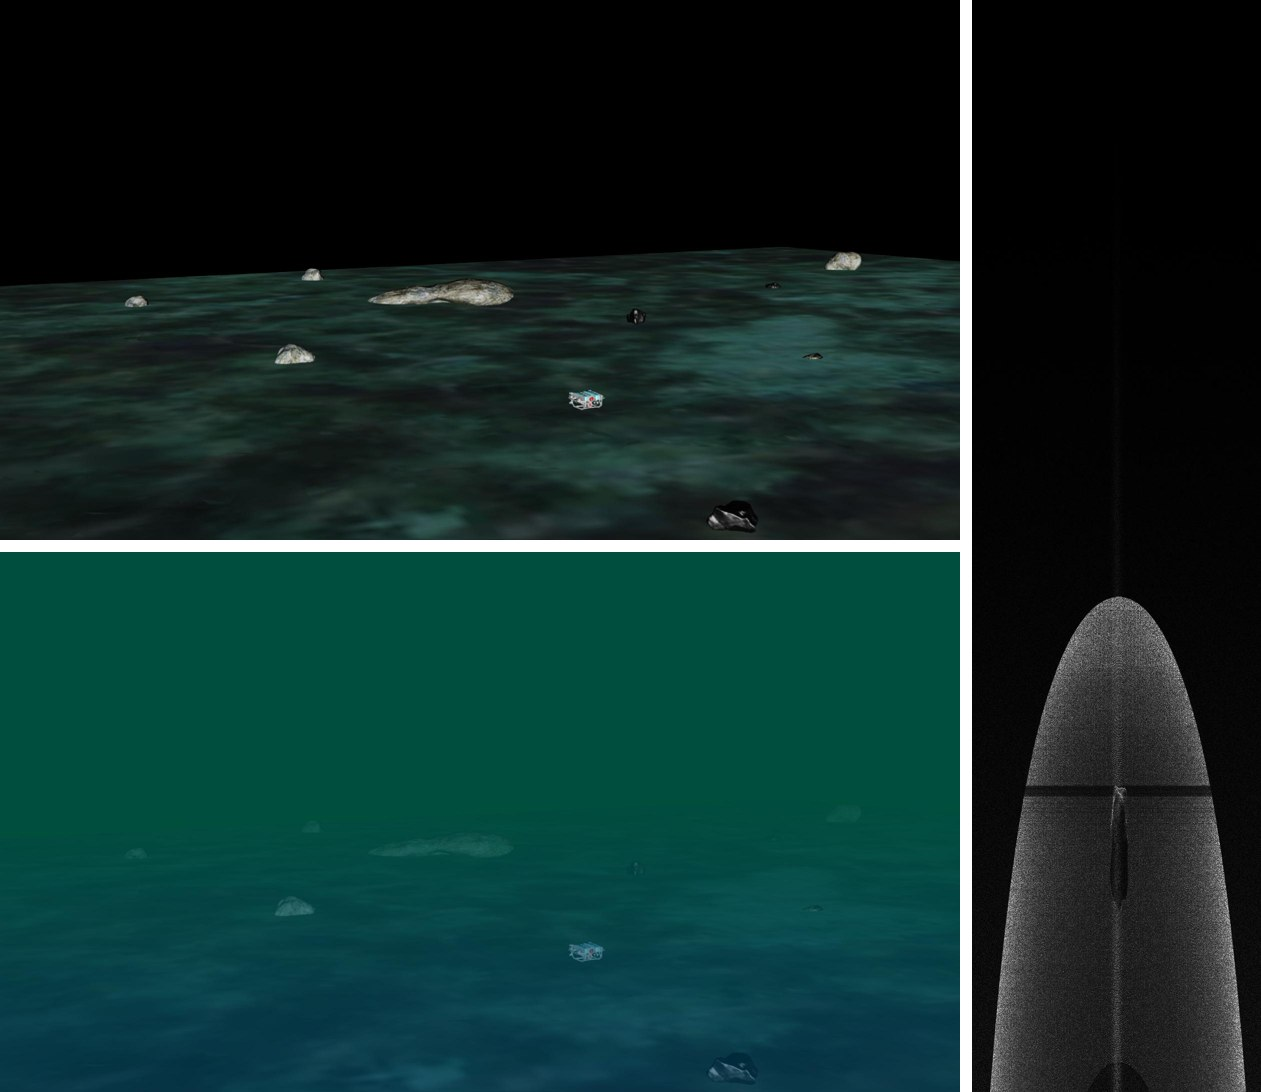
\includegraphics[width=0.48\textwidth]{saida_camera_sonar.jpg}
\caption{Saídas de uma gravação de 24/03/2026 com o mundo Prototipo1: câmera sem o efeito da água (em cima), a
mesma imagem com o modelo subaquático (embaixo) e a imagem em leque do sonar (direita).}
\end{figure}

Cada gravação é uma pasta com \arq{config.json}, \arq{stage.usd}, \arq{sensors\_extrinsics.json} (\novo{} desde 05/10:
transformação fixa corpo$\rightarrow$sensor de cada sensor ativo), \arq{occupancy\_map/}, \arq{occupancy\_map\_3d/} (no modo
\texttt{3d\_stack}) e \arq{state/} (\arq{common/}, \arq{sonar/raw/} e, depois do replay, \arq{rgb/}, \arq{depth/},
\arq{segmentation/}, \arq{normals/}). Poses ficam no referencial do mundo, em metros, com quatérnio na ordem
\texttt{[w, x, y, z]}.

%-------------------------------------------------------------------------------------------------------------
\section{World Builder}\label{sec:wb}
\arq{./scripts/launch\_world\_builder.sh} abre o Isaac só com a extensão \arq{omni.ext.patosim\_worldbuilder}, sem robô,
sensores ou gravação. Ela usa as mesmas funções de \arq{omni.ext.patosim.build} que o simulador usa, então o que
ela mostra vale para o Build.

\begin{table}[H]
\centering\small
\begin{tabularx}{\textwidth}{@{}lY@{}}
\toprule
Seção / botão & O que faz \\
\midrule
\botao{Load World (no robot)} & carrega o \arq{.usd} em \arq{/World/scene}, sem robô \\
\botao{Import Dataset Object} & lista \arq{plataforms/}, \arq{statues\_temples/}, \arq{scenario/}; posição, rotação, escala e
  refletividade; \botao{Insert Object Into World} \\
\botao{Check Semantic Classes} & conta os meshes sem os rótulos \texttt{class} e \texttt{reflectivity} que o sonar usa
  (sem eles o sonar usa um valor padrão, que parece certo na imagem mas está errado para o dataset) \\
\botao{Apply Default Reflectivity} & aplica a refletividade padrão aos meshes que não têm \\
\botao{Check Physics} & conta a geometria sem colisão (invisível para os raycasts do sonar e do LiDAR) \\
\botao{Apply Physics (Collisions)} & aplica colisão no mundo inteiro \\
\bottomrule
\end{tabularx}
\caption{World Builder. Nos testes, o Prototipo1 tinha 428 meshes sem classe nem refletividade e 234 com colisão. Depois
dos dois Apply, ficaram 428/428 com refletividade e 428/428 com colisão.}
\end{table}

As correções valem para o stage aberto. O \botao{Build} do simulador já aplica colisão no mundo todo e, com
\textbf{Sonar Refl.} marcado, a refletividade padrão. O World Builder serve para ver antes o que falta num mundo, por
exemplo meshes sem classe semântica, e corrigir o próprio arquivo do mundo.

%-------------------------------------------------------------------------------------------------------------
\section{Novidades em detalhe}\label{sec:detalhes}
\begin{table}[H]
\centering\small
\begin{tabularx}{\textwidth}{@{}p{3.5cm}YY@{}}
\toprule
Novidade & O que muda & Como usar \\
\midrule
\multicolumn{3}{@{}l}{\textit{09/11/2026}} \\
OceanSim dentro da extensão & imports \arq{omni.ext.patosim.oceansim}; o sonar não depende mais de uma cópia em
  \arq{app/extsUser} (na pdi\_mini\_3 essa cópia era de março) & nada a fazer; o teste confere de onde vem o código \\
Assets em dois layouts & \arq{assets/models/} ou \arq{assets/} & qualquer um dos dois \\
Mundo de exemplo & resolvido a partir do repositório & \botao{Use MHL Scene} ou \arq{PATOSIM\_DEV\_SCENE} \\
\midrule
\multicolumn{3}{@{}l}{\textit{24/10/2026}} \\
Navegação leve & sensores desligados por padrão & marcar em \botao{Robot Setup} antes de gravar \\
World Builder & launcher sem robô com checagens & \arq{launch\_world\_builder.sh} (seção~\ref{sec:wb}) \\
Testes de integração & cenário ROV completo, gravação curta e World Builder com o Isaac headless & seção~\ref{sec:testes} \\
\midrule
\multicolumn{3}{@{}l}{\textit{05/10/2026}} \\
Sonar \texttt{raw} & sem normalização por anel/quadro: a intensidade cai com a distância como no sensor real &
  padrão; \texttt{range}/\texttt{all} continuam como opções de visualização \\
Sonar bruto na gravação & \arq{state/sonar/raw/*.npy} gravado ao vivo, não só no replay & ligar o Sonar \\
LiDAR subaquático & perfis \texttt{insight\_nano} (0,13--2,5\,m), \texttt{insight\_micro} (0,13--7\,m) e \texttt{insight\_pro}
  (0,5--15\,m), com probabilidade de retorno $e^{-\alpha d}$ & \nome{lidar_range_profile} e
  \nome{lidar_attenuation_coeff} no \arq{Config} \\
Gamepad 6 DOF & novo cenário, com zona morta e expo & \nome{OceanSimROVGamepadTeleoperationScenario} \\
Extrínsecos & \arq{sensors\_extrinsics.json} em cada gravação & combinar com \nome{robot.position} e
  \nome{robot.orientation} \\
Mapa em camadas & \arq{OccupancyMapStack}: uma fatia 2D por banda de profundidade (Fig.~\ref{fig:bandas}) &
  \nome{occupancy_map_mode="3d_stack"} no \arq{Config}; a navegação ainda usa a fatia única \\
Escala de assets & compensa \texttt{metersPerUnit} do asset (assets em cm não ficam 100$\times$ maiores) & automático
  ao inserir objetos \\
\bottomrule
\end{tabularx}
\caption{Novidades, da mais recente para a mais antiga.}
\end{table}

\begin{figure}[H]
\centering

\includegraphics[width=0.78\textwidth]{mapa_3d_bandas.png}
\caption{Mapa de ocupação em camadas do Prototipo1, gerado no teste de integração: fatias centradas em
$z=-4$, $-2$ e $0$\,m (preto = ocupado). O fundo desse mundo fica em $z\approx0$\,m. Os corais atravessam o fundo
e aparecem na fatia de $-2$\,m. A fatia de $0$\,m corta o próprio fundo.}
\label{fig:bandas}
\end{figure}

%-------------------------------------------------------------------------------------------------------------
\section{Testes}\label{sec:testes}
\begin{lstlisting}[language=bash]
python3 -m pytest tests/unit                                          # 32 testes, sem Isaac
./app/python.sh tests/integration/run_gpu_integration_checks.py       # Isaac headless, 1 a 3 min
./app/python.sh tests/integration/run_worldbuilder_extension_check.py # Isaac headless, < 1 min
\end{lstlisting}
O teste de integração monta um cenário ROV com todos os sensores, grava uma sessão curta e confere os arquivos. Ele
também testa as ferramentas do World Builder, o mapa em camadas e o gamepad, e confirma que o código do sonar vem do
repositório. A comparação com uma gravação antiga só roda se ela existir (\arq{PATOSIM\_LEGACY\_RECORDING}).

% Resultados de 09/11/2026 (incluído em patosim_novidades.tex).
\begin{table}[H]
\centering\small
\begin{tabularx}{\textwidth}{@{}Ycc@{}}
\toprule
Checagem & \makecell{Esta máquina\\RTX 4070, driver 565} & \makecell{pdi\_mini\_3\\RTX 5060 Ti, driver 580} \\
\midrule
Testes unitários (\arq{tests/unit}) & 32/32 & 32/32 \\
Extensões, imports e código do sonar vindo do repositório & ok & ok \\
\arq{config.json} antigo (de antes dos campos novos) & ok & pulado (sem a gravação) \\
World Builder: checar e aplicar classes, refletividade e colisão; listar e inserir objetos &
  ok (428 meshes, 11 objetos) & ok (429 meshes, 12 objetos) \\
Cenário ROV com os 5 sensores, sonar \texttt{raw}, perfil \texttt{insight\_micro} do LiDAR & ok & ok \\
\textbf{Sinal do sonar} (intensidade diferente de zero) & \textbf{falha} & \textbf{falha} \\
Gravação ao vivo: extrínsecos, \arq{state/common}, sonar bruto, imagens do sonar & ok & ok \\
Mapa em camadas (3 fatias, salvo em disco) & ok & ok \\
Gamepad sem controle físico (comando zero) & ok & ok \\
Carregar gravação antiga no mesmo processo & crash do Isaac & pulado \\
Extensão World Builder sozinha (sem a principal, janela criada) & 6/6 & 6/6 \\
\midrule
Total do teste de integração & 25 ok, 1 falha, 1 crash & 26 ok (2 pulados), 1 falha \\
\bottomrule
\end{tabularx}
\caption{Resultados de 09/11/2026 com o código do \arq{main} (\arq{8c92c04}). A falha do sonar e o crash estão em
Limitações conhecidas.}
\end{table}


%-------------------------------------------------------------------------------------------------------------
\section{Limitações conhecidas}
\begin{itemize}
  \item \textbf{Spawn}: \arq{\_compute\_safe\_underwater\_spawn()} (\arq{build.py}) leva o ROV para 1\,m acima do objeto
        mais alto do mundo sempre que o ponto configurado cai dentro da caixa que envolve o mundo, o que é o caso
        normal. No Prototipo1 o fundo fica em $z\approx0$\,m e os objetos vão até 5,7\,m. O robô nasce em $z=6{,}7$\,m,
        e a profundidade padrão de \textbf{Depth (m)} ($-2$\,m) fica abaixo do fundo. Até a correção, posicione o
        robô com as teclas ou ajuste a profundidade ao mundo.
  % Incluído na lista de limitações de patosim_novidades.tex.
\item \textbf{Sonar no teste headless}: o teste de integração monta o sonar, roda o kernel e grava os arquivos,
      mas a intensidade sai zerada (mínimo = máximo = 0), nas duas máquinas. Isso acontece mesmo com o ROV 1,5\,m
      acima da primeira superfície abaixo dele (nesta máquina, o fundo do Prototipo1) e um objeto 3\,m à frente. Pela interface o sonar funciona (figura da seção~\ref{sec:uso}, gravação de 24/03). A causa no modo
      headless não foi isolada. Antes de uma gravação longa, confira o sonar na janela Sensor Preview.
\item \textbf{Checagem com a gravação antiga}: ao carregar a gravação de 24/03 no mesmo processo dos outros testes,
      o Isaac cai (crash nativo em \arq{omni.usd} ao criar o \arq{World} de novo). As outras checagens já estão
      salvas nesse ponto. Em máquinas sem essa gravação a checagem é pulada.

  \item \textbf{Path Planning}: a janela edita só o cenário terrestre herdado do MobilityGen. Os parâmetros do
        \nome{OceanSimROVPathFollowingScenario} ficam no código.
  \item \arq{oceansim/utils/asset\_path.json} aponta para \arq{/mnt/external/isaac/OceanSim\_assets}, que só existe numa
        máquina. Ele é só um caminho alternativo para o modelo do ROV (o principal vem dos assets do repositório).
        Para mudar: \arq{scripts/register\_oceansim\_assets.sh <pasta>} ou \arq{OCEANSIM\_ASSET\_PATH}.
  \item As cópias \arq{OceanSim}, \arq{OceanSim.bak} e \arq{PatoSIM} em \arq{app/extsUser} não são mais usadas pelo PatoSim
        e podem ficar onde estão.
\end{itemize}

\end{document}
